\documentclass[12pt]{article}
\usepackage[margin=1in]{geometry}
\usepackage[hidelinks]{hyperref}
\usepackage{enumitem}
\usepackage{booktabs}
\usepackage{array}
\usepackage{float}
\usepackage{amsmath}
\usepackage{tikz}
\usetikzlibrary{positioning, arrows.meta, shapes.geometric}
\setlist[itemize]{leftmargin=*, itemsep=2pt}
\setlist[enumerate]{leftmargin=*, itemsep=2pt}

\title{\textbf{Mealie High-Level Design}}
\author{System Design Document}
\date{\today}

\begin{document}
\maketitle

\section{Overview}
Mealie is a comprehensive meal planning and recipe discovery application designed to streamline the cooking experience for home chefs. It integrates recipe discovery, intelligent meal suggestions, inventory tracking, and automated grocery list generation into a unified platform. The system leverages an AI assistant (OAT) to provide personalised cooking guidance and uses preference-based recommendation algorithms to surface relevant recipes. The primary stakeholders are home cooks, meal planners, and individuals seeking to reduce food waste while improving their culinary repertoire. The one-sentence goal: \emph{Empower users to discover, plan, and execute meals efficiently through intelligent recipe management and inventory awareness.}

\section{Problem Statement}
Home cooking faces persistent friction points: recipe discovery is fragmented across multiple platforms, grocery planning is manual and error-prone, ingredient inventory management is neglected leading to food waste, and personalised meal suggestions require extensive user research. Users waste time searching for recipes that match their dietary preferences, manually transcribing ingredients to shopping lists, and frequently discovering expired items in their refrigerators. The absence of an integrated solution forces users to context-switch between recipe blogs, note-taking apps, and grocery list tools, reducing cooking efficiency and increasing decision fatigue. Resolving this gap enables streamlined meal planning, reduced food waste, and improved cooking confidence.

\section{Goals and Non-Goals}
\textbf{Goals}
\begin{itemize}
  \item Provide personalised recipe recommendations based on cuisine preferences, dietary restrictions, health goals, and available cooking time.
  \item Enable seamless transition from recipe discovery to grocery list generation with one-click ingredient addition.
  \item Track pantry inventory with expiration date monitoring and low-stock alerts.
  \item Offer AI-powered cooking assistance through conversational interface (Ask OAT).
  \item Maintain user preference profiles for consistent personalisation across sessions.
  \item Support barcode scanning for rapid inventory item entry.
\end{itemize}
\textbf{Non-Goals}
\begin{itemize}
  \item Real-time grocery delivery integration or price comparison (future phase).
  \item Nutritional analysis beyond calorie and macronutrient display (requires FDA-grade validation).
  \item Social features such as recipe sharing, community reviews, or cooking challenges.
  \item Meal kit subscription services or commercial partnerships.
  \item Multi-user household inventory sharing (deferred to v2.0).
\end{itemize}

\section{Requirements}
\textbf{Functional Requirements}
\begin{itemize}
  \item Authentication system must support OAuth integration (Google, Apple) with profile management.
  \item Preference survey must capture cuisine types, dietary restrictions, health goals, time availability, and grocery store preferences.
  \item Recipe catalogue must display title, image, cooking time, servings, calorie count, tags, ingredients list, and step-by-step instructions.
  \item Search functionality must filter recipes by keyword, cuisine, cooking time, and dietary compatibility.
  \item Grocery list must aggregate ingredients from multiple recipes, support custom item addition, and track completion status.
  \item Inventory system must record item name, quantity, expiration date, and category with visual expiration warnings.
  \item OAT assistant must process natural language queries and return contextual recipe suggestions or cooking advice.
\end{itemize}
\textbf{Non-Functional Requirements}
\begin{itemize}
  \item UI must render recipe grids and detail pages within $800$ms on standard 4G connections.
  \item Mobile-responsive design must support viewport widths from $320$px (mobile) to $1920$px (desktop).
  \item Preference data must persist across sessions with automatic synchronisation.
  \item System must gracefully degrade when external APIs (recipe sources, image services) are unavailable.
  \item Accessibility compliance with WCAG 2.1 Level AA for keyboard navigation and screen readers.
  \item Data privacy: no collection of personally identifiable information beyond authentication credentials.
\end{itemize}

\section{User Journey / Experience}
\begin{enumerate}
  \item User authenticates via Google/Apple OAuth and lands on account creation screen.
  \item System prompts for profile avatar selection and username entry.
  \item Preference survey collects cuisine preferences, dietary restrictions, health goals, cooking time availability, and preferred grocery stores across five progressive steps.
  \item Upon completion, user arrives at personalised dashboard displaying recipe recommendations sorted by Holistic Workability Index (HWI).
  \item User browses recipe grid, filters by tags, or initiates keyword search via dedicated search screen.
  \item Selecting a recipe navigates to detail view with expandable ingredients list and cooking instructions.
  \item User clicks ``Add to Grocery List'' to append all recipe ingredients; system navigates to grocery list with items pre-populated and grouped by category.
  \item User accesses inventory screen to manually add items or scan barcodes; system displays expiration warnings for items expiring within three days.
  \item User engages OAT assistant with queries like ``Quick 15-minute lunch ideas''; assistant returns recipe cards with inline preview and navigation to detail pages.
  \item Bottom navigation enables fluid transitions between Home, Search, Inventory, Grocery List, and Ask OAT screens.
\end{enumerate}

\section{System Architecture}
\subsection{Context Diagram}
\begin{figure}[H]
  \centering
  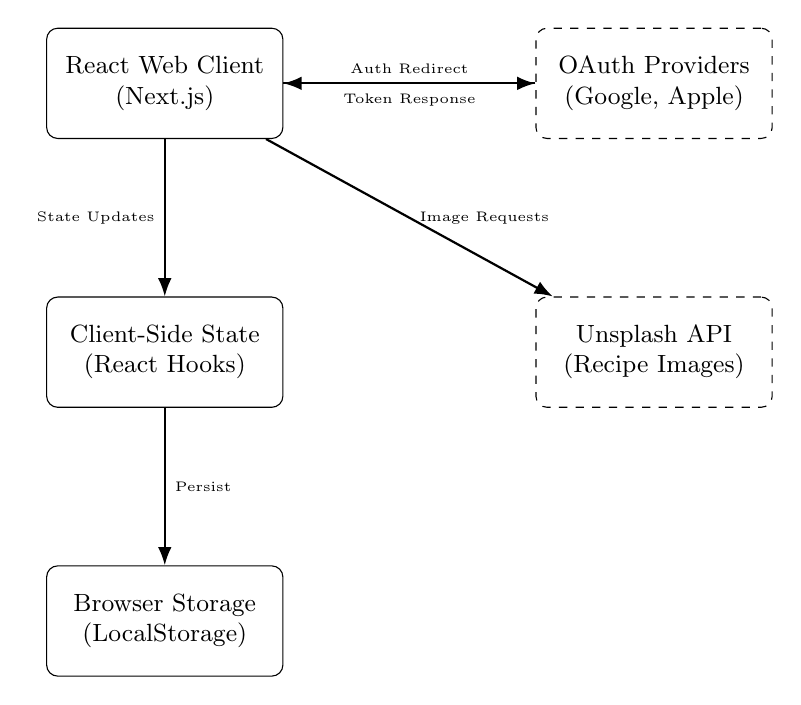
\begin{tikzpicture}[
    node distance=3.2cm,
    process/.style={rectangle, draw, rounded corners, minimum width=3cm, minimum height=1.4cm, align=center, font=\small},
    external/.style={rectangle, draw, rounded corners, dashed, minimum width=3cm, minimum height=1.4cm, align=center, font=\small},
    arrow/.style={-Latex, thick}
  ]
    \node[process] (client) {React Web Client\\(Next.js)};
    \node[external, right=of client] (auth) {OAuth Providers\\(Google, Apple)};
    \node[process, below=2cm of client] (state) {Client-Side State\\(React Hooks)};
    \node[external, below=2cm of auth] (images) {Unsplash API\\(Recipe Images)};
    \node[process, below=2cm of state] (storage) {Browser Storage\\(LocalStorage)};

    \draw[arrow] (client) -- node[above, font=\tiny]{Auth Redirect} (auth);
    \draw[arrow] (auth) -- node[below, font=\tiny]{Token Response} (client);
    \draw[arrow] (client) -- node[left, font=\tiny]{State Updates} (state);
    \draw[arrow] (state) -- node[right, font=\tiny]{Persist} (storage);
    \draw[arrow] (client) -- node[right, font=\tiny]{Image Requests} (images);
  \end{tikzpicture}
  \caption{System context showing client-side architecture with external OAuth and image services.}
\end{figure}

\subsection{Component Diagram}
\begin{itemize}
  \item \textbf{App Router}: Main orchestrator managing screen state transitions (SignIn, Account, Preferences, Dashboard, Recipe, Inventory, Grocery, Search, OAT).
  \item \textbf{Authentication Module}: Handles OAuth flow integration with Google/Apple providers, session management, and profile initialisation.
  \item \textbf{Preference Engine}: Multi-step survey component capturing user preferences with validation and progress tracking.
  \item \textbf{Recipe Catalogue}: Grid and detail view components displaying recipe data with tag-based filtering and search integration.
  \item \textbf{Grocery Manager}: List aggregation, item completion tracking, category grouping, and custom item entry interface.
  \item \textbf{Inventory Tracker}: CRUD operations for pantry items with expiration date monitoring, category filtering, and barcode scanning interface.
  \item \textbf{OAT Assistant}: Conversational UI with message history, quick prompt suggestions, and inline recipe card rendering.
  \item \textbf{Navigation Controller}: Bottom tab bar managing global navigation state and active screen highlighting.
\end{itemize}

\subsection{Data Flow Diagram}
\begin{enumerate}
  \item User initiates OAuth login $\rightarrow$ redirects to provider $\rightarrow$ receives authentication token $\rightarrow$ creates local session.
  \item Preference survey collects multi-step responses $\rightarrow$ validates completeness $\rightarrow$ persists to localStorage $\rightarrow$ triggers dashboard navigation.
  \item Dashboard requests recipe data $\rightarrow$ filters by user preferences $\rightarrow$ sorts by recommendation score $\rightarrow$ renders grid with lazy-loaded images.
  \item Recipe detail ``Add to Grocery List'' action $\rightarrow$ extracts ingredients array $\rightarrow$ merges with existing grocery items $\rightarrow$ updates localStorage $\rightarrow$ navigates to grocery screen.
  \item Inventory item creation $\rightarrow$ validates required fields $\rightarrow$ calculates expiration warnings $\rightarrow$ persists to localStorage $\rightarrow$ updates inventory list view.
  \item OAT query submission $\rightarrow$ parses natural language input $\rightarrow$ matches against recipe database $\rightarrow$ returns ranked suggestions with preview cards.
\end{enumerate}

\section{Data Model}
\textbf{Entities}
\begin{itemize}
  \item \textbf{User Profile}: `userId`, `username`, `avatarEmoji`, `preferences` (cuisines[], dietary[], healthGoals[], cookingTime, groceryStore), `createdAt`.
  \item \textbf{Recipe}: `recipeId`, `title`, `image`, `time`, `servings`, `calories`, `description`, `tags[]`, `ingredients[]` (item, amount), `steps[]`, `category`.
  \item \textbf{Grocery Item}: `itemId`, `name`, `quantity`, `category`, `checked`, `fromRecipe` (optional reference), `addedAt`.
  \item \textbf{Inventory Item}: `itemId`, `name`, `quantity`, `expiryDate`, `daysUntilExpiry`, `category`, `addedAt`, `lastUpdated`.
  \item \textbf{OAT Message}: `messageId`, `type` (user/assistant), `content`, `suggestions[]` (recipe references), `timestamp`.
\end{itemize}
\textbf{Relationships}
\begin{itemize}
  \item User Profile (1) $\leftrightarrow$ (N) Grocery Items: One user maintains multiple grocery list entries.
  \item User Profile (1) $\leftrightarrow$ (N) Inventory Items: One user tracks multiple pantry items.
  \item Recipe (1) $\rightarrow$ (N) Grocery Items: Recipe ingredients generate multiple grocery list entries via ``Add to List'' action.
  \item OAT Message (1) $\rightarrow$ (N) Recipe Suggestions: Assistant responses embed multiple recipe recommendations.
\end{itemize}

\section{Implementation Approach}
\begin{itemize}
  \item \textbf{Client-Side State Management}: React hooks (`useState`) manage screen transitions, form inputs, and UI interactions without external state libraries to reduce complexity.
  \item \textbf{LocalStorage Persistence}: User preferences, grocery lists, and inventory data persist to browser localStorage with JSON serialisation for offline-first capability.
  \item \textbf{Modular Component Architecture}: Each screen (Dashboard, Search, Inventory, etc.) implemented as isolated functional component with clear prop interfaces for maintainability.
  \item \textbf{Lazy Image Loading}: Recipe images fetched on-demand via Unsplash API with fallback placeholders to optimise initial page load performance.
  \item \textbf{Responsive Design}: Tailwind CSS utility classes enable mobile-first responsive layouts without custom media queries.
  \item \textbf{Accessibility Patterns}: Semantic HTML elements, ARIA labels, keyboard navigation support, and focus management ensure screen reader compatibility.
  \item \textbf{Trade-off Justification}: Prioritised rapid prototyping and frontend-only implementation over backend infrastructure to validate user experience before investing in server architecture.
\end{itemize}

\section{Platform and Infrastructure}
\begin{itemize}
  \item \textbf{Frontend Framework}: React 18 with TypeScript for type-safe component development.
  \item \textbf{Build System}: Vite bundler with hot module replacement for sub-second dev server refresh.
  \item \textbf{Styling}: Tailwind CSS v4.0 with custom design tokens (emerald primary palette, neutral grays, rounded-2xl radius standard).
  \item \textbf{Icon Library}: Lucide React for consistent icon design system (outlined style).
  \item \textbf{Image Service}: Unsplash API for high-quality recipe photography with attribution compliance.
  \item \textbf{Hosting}: Static site deployment via Vercel edge network with automatic HTTPS and CDN caching.
  \item \textbf{Development Environment}: Node.js 18+, npm package manager, ESLint for code quality, Prettier for formatting.
\end{itemize}

\section{Security and Access Control}
\begin{itemize}
  \item \textbf{Authentication}: OAuth 2.0 integration with Google and Apple identity providers eliminates password management risks.
  \item \textbf{Data Privacy}: No personally identifiable information collected beyond OAuth-provided name and email; no analytics tracking implemented.
  \item \textbf{Client-Side Storage}: LocalStorage isolation prevents cross-site data access; all data scoped to application origin.
  \item \textbf{API Key Protection}: Unsplash API keys configured with HTTP referrer restrictions to prevent unauthorised usage.
  \item \textbf{Content Security Policy}: Strict CSP headers prevent XSS attacks via inline script blocking and resource whitelisting.
  \item \textbf{HTTPS Enforcement}: All production traffic encrypted via TLS 1.3 with automatic certificate renewal.
\end{itemize}

\section{Trade-Offs and Design Decisions}
\begin{center}
\begin{tabular}{>{\bfseries}p{0.23\linewidth} p{0.32\linewidth} p{0.32\linewidth}}
\toprule
Decision & Trade-Off & Rationale \\
\midrule
Client-only architecture & No multi-device sync & Faster MVP delivery without backend infrastructure \\
LocalStorage over database & Data loss on cache clear & Eliminates hosting costs while maintaining UX \\
Static recipe catalogue & No user-generated content & Ensures quality control and reduces moderation burden \\
Mock OAT responses & Limited conversational depth & Demonstrates UI/UX without LLM API integration costs \\
Single-user focus & No household sharing & Simplifies data model and access patterns \\
Manual barcode scanning UI & No actual scanning logic & Provides interface foundation for future implementation \\
\bottomrule
\end{tabular}
\end{center}

\section{Future Enhancements}
\begin{itemize}
  \item \textbf{Backend Integration}: Supabase or Firebase backend for multi-device synchronisation and real-time updates.
  \item \textbf{Real LLM Integration}: OpenAI GPT-4 or Anthropic Claude for dynamic OAT conversational responses.
  \item \textbf{Barcode Scanning}: React Native Camera integration or Web Barcode Detection API for actual product scanning.
  \item \textbf{Nutritional Analysis}: Integration with USDA FoodData Central API for detailed macro/micronutrient breakdowns.
  \item \textbf{Meal Planning Calendar}: Weekly/monthly calendar view with drag-and-drop recipe scheduling.
  \item \textbf{Recipe Import}: Parse recipe URLs from popular food blogs using schema.org Recipe markup.
  \item \textbf{Smart Notifications}: Push notifications for expiring inventory items and meal planning reminders.
  \item \textbf{Social Features}: Recipe collections, family sharing, and collaborative grocery lists.
  \item \textbf{Grocery Store Integration}: API partnerships with Instacart, Amazon Fresh for one-click ordering.
  \item \textbf{Advanced Search}: Faceted filtering by ingredient inclusion/exclusion, cooking method, equipment requirements.
\end{itemize}

\section{Algorithmic Components}
\subsection{Recipe Recommendation Scoring}
The system employs a weighted scoring function to rank recipes based on user preferences:
\begin{equation}
  S_{\text{recipe}} = w_c \cdot M_{\text{cuisine}} + w_d \cdot M_{\text{dietary}} + w_t \cdot M_{\text{time}} + w_h \cdot M_{\text{health}}
\end{equation}
where $w_i$ represents preference weights and $M_i$ are binary match indicators (1 if recipe satisfies criterion, 0 otherwise). Default weights: $w_c = 0.35$, $w_d = 0.30$, $w_t = 0.20$, $w_h = 0.15$.

\subsection{Inventory Expiration Prioritisation}
Items displayed with urgency indicators based on days until expiry:
\begin{equation}
  \text{Priority} = \begin{cases}
    \text{Critical} & \text{if } d \leq 1 \\
    \text{Warning} & \text{if } 1 < d \leq 3 \\
    \text{Normal} & \text{if } d > 3
  \end{cases}
\end{equation}
where $d$ represents days until expiration. Critical items trigger visual alerts and appear first in sorted lists.

\section{Conclusion}
Mealie delivers an integrated meal planning experience that addresses fragmented recipe discovery, manual grocery list management, and neglected inventory tracking through a cohesive, user-centric design. The client-side architecture prioritises rapid iteration and deployment simplicity while maintaining extensibility for future backend enhancements. By emphasising intuitive navigation, personalised recommendations, and AI-assisted cooking guidance, the system reduces decision fatigue and enables confident meal preparation. The modular component design and clear data models establish a foundation for scaling to multi-user scenarios, real-time synchronisation, and advanced nutritional analysis.

\section{Appendix}
\subsection{Screen Navigation Map}
\begin{verbatim}
SignIn → AccountDetails → PreferenceSurvey → Dashboard
                                                ├── RecipeDetail
                                                ├── Search → SearchResults → RecipeDetail
                                                ├── Inventory → AddItem / ScanBarcode
                                                ├── GroceryList → AddGroceryItem
                                                └── AskOAT → RecipeDetail
\end{verbatim}

\subsection{Sample Data Structures}
\textbf{Recipe Object (JSON)}
\begin{verbatim}
{
  "id": 1,
  "title": "Creamy Carbonara",
  "time": "25 min",
  "servings": 4,
  "calories": 540,
  "tags": ["Italian", "Quick"],
  "ingredients": [
    {"item": "Spaghetti", "amount": "400g"},
    {"item": "Pancetta", "amount": "200g"}
  ],
  "steps": ["Boil pasta...", "Fry pancetta..."]
}
\end{verbatim}

\textbf{Inventory Item (JSON)}
\begin{verbatim}
{
  "id": 1,
  "name": "Milk",
  "quantity": "1L",
  "expiryDate": "2025-12-05",
  "daysUntilExpiry": 3,
  "category": "Dairy"
}
\end{verbatim}

\subsection{Technology Stack Summary}
\begin{itemize}
  \item React 18.3+ (UI framework)
  \item TypeScript 5.0+ (type safety)
  \item Tailwind CSS 4.0 (styling)
  \item Lucide React (icons)
  \item Unsplash API (images)
  \item Vite (build tool)
  \item Vercel (hosting)
\end{itemize}

\subsection{API Endpoints (Planned)}
\begin{itemize}
  \item \texttt{GET /api/recipes?cuisine=\{type\}\&time=\{max\}} — Filtered recipe list
  \item \texttt{GET /api/recipes/\{id\}} — Recipe detail with ingredients/steps
  \item \texttt{POST /api/grocery} — Add items to user's grocery list
  \item \texttt{GET /api/inventory} — Retrieve user's pantry items
  \item \texttt{POST /api/inventory} — Add/update inventory item
  \item \texttt{POST /api/oat/query} — Submit natural language cooking query
\end{itemize}

\end{document}
